\section{TreeTiler}
\label{sec:tiler}

The work showed on \cite{tree_tiler} presents a framework, \treetiler, that can be used to refactor Java code at runtime. Given a Java application source code as input, \treetiler will try to detect a recursive data structure. It will then look for a recursive method that performs a recursive traversal on that structure.

The JastAdd framework is employed to analyse and refactor the Java input at compile time, generating the output consisting of the same program with the applied optimizations, which are described here.

\subsection{Optimizations}
\label{sec:optim}

The techniques employed by \treetiler deal with the way a recursive structure is traversed. Even though it is commonly an irregular structure, some techniques can be applied to exploit locality when multiple traversals are done. In this report, the techniques used were the Spatial Sort and Point Blocking. An Auto Tuner is also added to the Java code by \treetiler. This Tuner tries to find the best parameters for the optimizations, which sometimes are input dependent and cannot be evaluated at compile time.

\subsubsection{Sorting}
\label{sec:optim:sort}

Traversing an irregular structure requires loading from memory the elements of the structure which, due to their irregular nature, can not be obtained in an optimized way through prefetching. Also, the elements of this structure which are consecutively accessed (especially in parallel) will most probably lie in distinct cache lines, hurting locality.

By changing the order of accesses in these structures, so that domain objects with similar traversal patterns become consecutive, temporal locality is improved as the elements a given object will touch are already likely to have been touched by the previous one.

Sorting these objects in applications where the domain refers to a notion of space can be performed using space-filling curves\footnote{A curve which touches every object in the domain only once. Examples of these curves are the Peano and Hilbert curves.} (for algorithms in the space domain like Barnes-hut). The examples described in this document use the CGAL library, implementing the traits required for spatial sorting in 3D.

\begin{figure}[!htp]
	\centering
	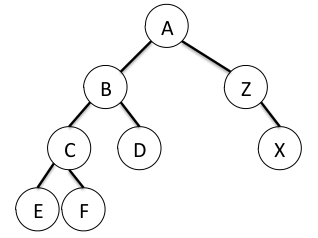
\includegraphics[width=0.4\columnwidth]{pointblocking_tree}
	\caption{A sample tree}
	\label{fig:tree}
\end{figure}

\begin{figure}[!htp]
	\centering
	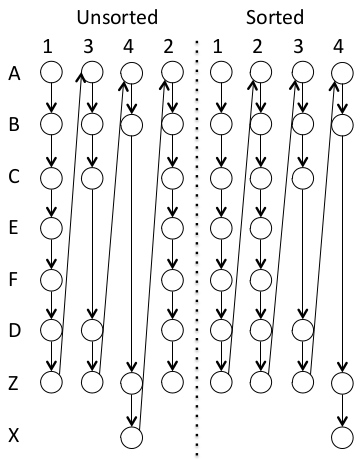
\includegraphics[width=0.6\columnwidth]{pointblocking_sort}
	\caption{Spatial Sort transformation applied to traversal of tree shown in \cref{fig:tree}}
	\label{fig:sort}
\end{figure}

\paragraph{Limitations:}
Processing objects in an order which brings similar traversals closer in time only brings improvements when the traversal itself fits in cache. This will allow subsequent objects to take advantage of the acceleration structure elements already visited by previous objects. For sufficiently deep traversals, when the subsequent objects traverse the structure, the first elements have already been evicted from cache. \cite{tree_tiler} already shows that as the traversal size increases, the locality improvements gained from the Sorting optimization decrease drastically.

\subsubsection{Blocking}
\label{sec:optim:block}

Since it is likely that geometrically closer points also follow a similar traversal, which is the basis for the Spatial Sort optimization, it is also likely that those points can be processed in blocks, rather than one at a time, thus taking advantage of locality, and preventing the traversal from being evicted too soon from cache.

Instead of traversing the structure for a single point, and iteratively switching points, the new strategy takes advantage of the premise that Spatial Sort rearranges points so that a small subset of points is likely to be geometrically close to each other. This subset is grouped into a block, and the tree is traversed for that block at the same time.

The root node of the structure is processed for all points of the block. If necessary (depending on the algorithm), if the paths of each point in the block diverge at a given node, it may be necessary to split the block into smaller blocks, each one going to a different node. Given the geometrical proximity, this is only more likely to occur at the last levels of the structure, allowing for some locality to still be gained in the previous levels.

\Cref{fig:sort} illustrates the execution order of a point blocked implementation, compared to the non blocked, sorted implementation.

\begin{figure}[!htp]
	\centering
	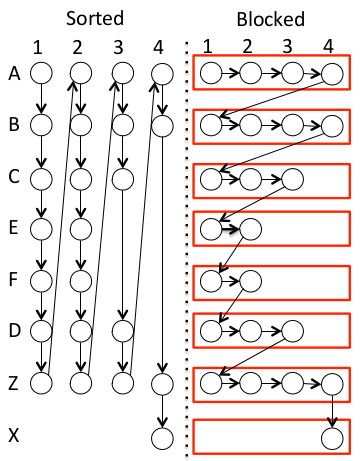
\includegraphics[width=0.6\columnwidth]{pointblocking_blocks}
	\caption{Point Blocking transformation}
	\label{fig:sort}
\end{figure}

It is intuitive to notice that this strategy is only good if the points within a block are likely to follow a similar traversal path, otherwise too much divergence will hinder performance much like the original strategy.

\subsubsection{Auto Tuner}
\label{sec:optim:tuner}
The optimal block size is dependent on both hardware and algorithm details, but it may also be input dependent. The optimal block size for a Barnes-Hut implementation might not be the same as the ideal block size for a Ray Tracing application. Given that, a generic framework like \treetiler must not make assumptions about the algorithm and the input only at compile time.

For that reason, \treetiler installs an AutoTuner in the output code. This AutoTuner will perform a small sample (possibly selected randomly) of block iterations, and evaluate their performance at runtime.
Tipically, it is expected that a block size too small will yield bad results, possibly even worse than the original version, due to large overhead of the additional instructions for the point blocking, and because of the fact that misses in the tree occur between each block. In contrast, a block size too big wil not fit in cache, and misses will occur in the block items instead.

A sweet spot is expected to occur where the block size is near ideal value, meaning the block size is large enough to avoid cache misses in the tree, but still small enough to fit in cache.

The AutoTuner might then start at a small block size, and process the chosen samples, measuring the average traversal time for each subsequent block size. The time is expected to reduce until the sweet spot is reached, at which point the time will start to increase again.
When this happens, the best block size is the one that yielded the lowest runtime.
